\documentclass[paper,twocolomn]{geophysics}
%\documentclass[manuscript]{geophysics}
%\documentclass[manuscript,endfloat]{geophysics}
\usepackage{amsmath,amssymb,amsfonts,graphicx,subfigure,bm,yfonts,hyperref,cleveref,xcolor}
\usepackage{rotating}
%\usepackage[outdir=./]{epstopdf}

\usepackage{multirow}


%%%%%%%%%                              DEFINITIONS START

\def\cpar{$C_{ij},\rho$ parameterization~}
\def\hpar{h-parameterization~}

\newcommand{\todo}[1]{{\textbf {\color{red} #1}}}
\newcommand{\done}[1]{{\bf {\color{green} #1}}}
\newcommand{\connect}{{\textbf{\color{red} $<-$ Connect $->$ }}}


\def\rmrk#1{{\textbf{[[#1]]}}}
\def\rmrkok#1{}
%\def\eqref#1{\ref{#1}}
\def\eqrf#1{equation~\eqref{eq:#1}}
%\def\eqref#1{equation~\ref{eq:#1}}
\def\eq{equation~}
\def\figref#1{Figure~\ref{fig:#1}}
\def\figrefp#1{(Figure~\ref{fig:#1})}

\def\fref#1{\ref{#1}}

\def\rhoK{\hat{\rho}}
\def\cK{\hat{c}}


%\def\rmrk#1{{[\textcolor[rgb]{0,0,0.8}{#1}]}} % [blue]
%\def\rmrkm#1{{\textbf{[[\textcolor[rgb]{{1.00,0.00,0.00}}{#1}]]}}}
% _____________________________________________________________________________
\def\mainauthor{Vladimir Kazei}
\def\coauthorb{Ekkehart Tessmer}
\def\coauthorc{}%Zedong Wu
\def\coauthora{Tariq Alkhalifah}
% - my definitions==============================================================================================

\def\DP{Diffraction-based radiation 
patterns }
\def\dP{diffraction-based radiation 
patterns }

\def\nt{N}
\newcommand{\Mod}[1]{\ (\mathrm{mod}\ #1)}
\def\dv{\mathbf{d}}
\def\Amat{\mathbb{A}}
\def\Rmat{\mathbb{R}}
\def\Umat{\mathbb{U}}
\def\Smat{\mathbb{S}}
\def\Vmat{\mathbb{V}}
\def\SF{R}
\def\xv{\mathbf{x}}
\def\mv{\mathbf{m}}
%\def\tmul{\otimes}
\def\tmul{}
\def\cv{\mathbf{c}}

\def\sp{\varsigma}
\def\spv{\bm{\sp}}
\def\gp{\xi}
\def\gpv{\bm{\gp}}

\newcommand{\nmz}[1]{\mathbf{\bar{\text{$#1$}}}}
%\def\nmz#1{\mathbf{\bar #1}}

\def\Uv{\mathbf{U}}
\def\kv{\mathbf{k}}
\def\sv{\mathbf{s}}
\def\svn{\mathbf{\bar{\sv}}}
\def\Sv{\mathbf{S}}
\def\Gv{\mathbf{G}}
\def\Cv{\mathbf{C}}
\def\ev{\mathbf{e}}
\def\gv{\mathbf{g}}
\def\gvn{\mathbf{\bar{\gv}}}
\def\Av{\mathbf{A}}
\def\Bv{\mathbf{B}}
\def\uv{\mathbf{u}}
\def\rv{\mathbf{r}}
\def\dxv{\Delta \mathbf{x}}
\def\Kv{\mathbf{K}}
\def \cost{ \cos \frac{\theta}{2}}
%\newcommand{\sdot}{\mathbf{\bullet}}

\newcommand{\sdot}{{WI-WS, \delta \mv}}

\newcommand{\inty}{\int\limits_{-\infty}^{+\infty}}
\newcommand{\intyt}{\inty\inty\inty}
\newcommand{\intyV}{\int\limits_{V}}

\def\Rp{\mathcal{R}}
\def\Dp{\mathcal{D}}
\def\Tp{\mathcal{T}}
%\def\Cp{\mathcal{C}}
\def\Sp{\mathcal{S}}

% - Tariq's definitions begin here ==============================================================================
\def\beq{\begin{eqnarray}}
\def\eeq{\end{eqnarray}}

\def\mmbx#1{{\mathbf{#1}}}

\def\phi{\varphi}

\def\Vv{\mmbx{V}}
\def\gammav{\pmb{\gamma}}
\def\epsv{\pmb{\eps}}
\def\deltav{\pmb{\delta}}
\def\etav{\pmb{\eta}}

\def\v{V}
\def\rhov{\pmb{\rho}}
\def\r{\mmbx{r}}
\def\k{\mmbx{k}}

\def\d{\text{d}}
\def\c{\mmbx{c}}
\def\e{\mmbx{e}}
\def\m{\mmbx{m}}
\def\x{\mmbx{x}}
\def\xs{\x_s}
\def\xr{\x_r}
\def\L{\mmbx{L}}
\def\p{\mmbx{p}}
\def\q{\mmbx{q}}

\def\La{{\cal L}}
\def\tf{\tilde{f}}
\def\tA{\tilde{A}}
\def\ttau{\tilde{\tau}}
\def\y{\mmbx{y}}
\def\z{\mmbx{z}}

\def\tm{\tilde{m}}
\def\tr{\tilde{r}}
\def\tw{\tilde{w}}
\def\tv{\tilde{v}}
\def\tp{\tilde{p}}
\def\tq{\tilde{q}}

\def\a{\mmbx{a}}
\def\H{\mmbx{H}}
\def\g{\mmbx{g}}
\def\W{\mmbx{W}}

\def\eps{\varepsilon}

\def\La{{\cal L}}

\def\tlambda{\tilde{\lambda}}
\def\tw{\tilde{w}}

\def\rvn{r_{v_n}}
\def\rvh{r_{v_h}}
\def\rrho{r_\rho}
\def\rdel{r_\delta}
\def\reta{r_\eta}
\def\reps{r_\eps}


\def\Re{{{\cal{R}}_e}}

\newcommand{\pd}[2]{\frac{\partial #1}{\partial #2}}

%==============================================end of Tariq's notation=========================================


%%%%%%%%%								DEFINITIONS END
\newcommand{\mylabel}[1]{\label{#1}}
\newcommand{\myrf}[1]{\ref{#1}}

%%\newcommand{\plot}[3]{
%	\begin{figure}
%		\center
%		\includegraphics[#2]{Fig/#1}
%		\caption{#3}
%		\label{fig:#1}
%	\end{figure}
%}

\newcommand{\aplot}[3]{
	\begin{figure}[htbp!]
		\center
		\includegraphics[#2]{#1}
		\caption{#3}
		\label{fig:#1}
	\end{figure}
}

\newcommand{\twplot}[3]{
	\begin{figure}
		\centering
		\subfigure[]{\includegraphics[width=0.4\columnwidth]{Fig/#1}
			\label{fig:#1}}
		\hspace*{-0.01\columnwidth}
		\subfigure[]{\includegraphics[width=0.55\columnwidth]{Fig/#2}
			\label{fig:#2}}
		\caption{#3}
		%\label{fig:#1}
	\end{figure}
}

\newcommand{\tplot}[4]{
	\begin{figure}
		\centering
		\subfigure[]{\includegraphics[width=0.3\columnwidth]{Fig/#1}
			\label{fig:#1}}
		\vspace*{-0.01\columnwidth}
		\subfigure[]{\includegraphics[width=0.3\columnwidth]{Fig/#2}
			\label{fig:#2}}
		\vspace*{-0.01\columnwidth}
		\subfigure[]{\includegraphics[width=0.3\columnwidth]{Fig/#3}
			\label{fig:#3}}
		\caption{#4}
		\label{fig:#1_#3}\label{fig:#1_Full}
	\end{figure}
}
\newcommand{\tplott}[4]{
	\begin{figure}
		\centering
		\subfigure[]{\includegraphics[width=0.2\columnwidth]{Fig/#1}
			\label{fig:#1}}
		\vspace*{-0.01\columnwidth}
		\subfigure[]{\includegraphics[width=0.4\columnwidth]{Fig/#2}
			\label{fig:#2}}
		\vspace*{-0.01\columnwidth}
		\subfigure[]{\includegraphics[width=0.3\columnwidth]{Fig/#3}
			\label{fig:#3}}
		\caption{#4}
		\label{fig:#1_#3}\label{fig:#1_Full}
	\end{figure}
}
\newcommand{\tplotv}[4]{
	\begin{figure}
		\centering
		\subfigure[]{\includegraphics[width=0.49\columnwidth]{Fig/#1}
			\label{fig:#1}}
		\vspace*{-0.01\columnwidth}
		\subfigure[]{\includegraphics[width=0.49\columnwidth]{Fig/#2}
			\label{fig:#2}}
		\vspace*{-0.01\columnwidth}
		\subfigure[]{\includegraphics[width=0.49\columnwidth]{Fig/#3}
			\label{fig:#3}}
		\caption{#4}
		\label{fig:#1_#3}\label{fig:#1_Full}
	\end{figure}
}

\newcommand{\ffplot}[5]{
	\begin{figure}
		\centering
		\subfigure[]{\includegraphics[height=0.47\columnwidth]{Fig/#1}
			\label{fig:#1}}
		\hspace*{0.01\columnwidth}
		\subfigure[]{\includegraphics[height=0.47\columnwidth]{Fig/#2}
			\label{fig:#2}}
		\hspace*{-0.01\columnwidth}
		\subfigure[]{\includegraphics[height=0.47\columnwidth]{Fig/#3}
			\label{fig:#3}}
		\hspace*{0.01\columnwidth}
		\subfigure[]{\includegraphics[height=0.47\columnwidth]{Fig/#4}
			\label{fig:#4}}
		\caption{#5}
		\label{fig:#1:#4}\label{fig:#1_Full}
		\vspace*{-0.03\columnwidth}
	\end{figure}
}

\newcommand{\fplot}[5]{
	\begin{figure}
		\centering
		\subfigure[]{\includegraphics[height=0.27\columnwidth]{Fig/#1}
			\label{fig:#1}}
		\hspace*{0.01\columnwidth}
		\subfigure[]{\includegraphics[height=0.27\columnwidth]{Fig/#2}
			\label{fig:#2}}
		\hspace*{-0.01\columnwidth}
		\subfigure[]{\includegraphics[height=0.27\columnwidth]{Fig/#3}
			\label{fig:#3}}
		\hspace*{0.01\columnwidth}
		\subfigure[]{\includegraphics[height=0.27\columnwidth]{Fig/#4}
			\label{fig:#4}}
		\caption{#5}
		\label{fig:#1:#4}\label{fig:#1_Full}
		\vspace*{-0.03\columnwidth}
	\end{figure}
}

\newcommand{\splot}[7]{
	\begin{figure}
		\centering
		\subfigure[]{\includegraphics[height=0.27\columnwidth]{Fig/#1}
			\label{fig:#1}}
		\hspace*{0.01\columnwidth}
		\subfigure[]{\includegraphics[height=0.27\columnwidth]{Fig/#2}
			\label{fig:#2}}
		\hspace*{-0.01\columnwidth}
		\subfigure[]{\includegraphics[height=0.27\columnwidth]{Fig/#3}
			\label{fig:#3}}
		\hspace*{0.01\columnwidth}
		\subfigure[]{\includegraphics[height=0.27\columnwidth]{Fig/#4}
			\label{fig:#4}}
		\subfigure[]{\includegraphics[height=0.27\columnwidth]{Fig/#5}
			\label{fig:#5}}
		\subfigure[]{\includegraphics[height=0.27\columnwidth]{Fig/#6}
			\label{fig:#6}}
		\caption{#7}
		\label{fig:#1:#6}\label{fig:#1_Full}
		\vspace*{-0.03\columnwidth}
	\end{figure}
}

\newcommand{\fiPlot}[6]{
	\begin{figure}
		\centering
		\subfigure[]{\includegraphics[width=0.31\columnwidth]{Fig/#1}
			\label{fig:#1}}
		\hspace*{-0.01\columnwidth}
		\subfigure[]{\includegraphics[width=0.31\columnwidth]{Fig/#2}
			\label{fig:#2}}
		\hspace*{-0.01\columnwidth}
		\subfigure[]{\includegraphics[width=0.31\columnwidth]{Fig/#3}
			\label{fig:#3}}
		\hspace*{-0.01\columnwidth}
		\subfigure[]{\includegraphics[width=0.33\columnwidth]{Fig/#4}
			\label{fig:#4}}
		\subfigure[]{\includegraphics[width=0.33\columnwidth]{Fig/#5}
			\label{fig:#5}}
		\caption{#6}
		\label{fig:#1:#5}\label{fig:#1_Full}
	\end{figure}
}

\newcommand{\dplot}[3]{
	\begin{figure}
		\centering
		\subfigure[]{\includegraphics[height=0.45\columnwidth]{Fig/#1}
			\label{fig:#1}}
		\hspace*{-0.01\columnwidth}
		\subfigure[]{\includegraphics[height=0.45\columnwidth]{Fig/#2}
			\label{fig:#2}}
		\vspace*{-0.01\columnwidth}
		\caption{#3}
		\label{fig:#1:#2}\label{fig:#1_Full}
	\end{figure}
}

\newcommand{\ddplot}[3]{
	\begin{figure}
		\centering
		\subfigure[]{\includegraphics[width=0.7\columnwidth]{Fig/#1}
			\label{fig:#1}}
		\hspace*{-0.01\columnwidth}
		\subfigure[]{\includegraphics[width=0.99\columnwidth]{Fig/#2}
			\label{fig:#2}}
		\vspace*{-0.01\columnwidth}
		\caption{#3}
		\label{fig:#1_#2}\label{fig:#1_Full}
	\end{figure}
}

\def\ewidth{0.4}


\newcommand{\eplot}[9]{
	\begin{figure}
		\centering
		\subfigure[]{\includegraphics[width=\ewidth\columnwidth]{Fig/#1}
			\label{fig:#1}}
		\hspace*{-0.01\columnwidth}
		\subfigure[]{\includegraphics[width=\ewidth\columnwidth]{Fig/#2}
			\label{fig:#2}}
		\hspace*{-0.01\columnwidth}
		\subfigure[]{\includegraphics[width=\ewidth\columnwidth]{Fig/#3}
			\label{fig:#3}}
		\hspace*{-0.01\columnwidth}
		\subfigure[]{\includegraphics[width=\ewidth\columnwidth]{Fig/#4}
			\label{fig:#4}}
		\hspace*{-0.01\columnwidth}
		\subfigure[]{\includegraphics[width=\ewidth\columnwidth]{Fig/#5}
			\label{fig:#5}}
		\hspace*{-0.01\columnwidth}
		\subfigure[]{\includegraphics[width=\ewidth\columnwidth]{Fig/#6}
			\label{fig:#6}}
		\hspace*{-0.01\columnwidth}
		\subfigure[]{\includegraphics[width=\ewidth\columnwidth]{Fig/#7}
			\label{fig:#7}}
		\hspace*{-0.01\columnwidth}
		\subfigure[]{\includegraphics[width=\ewidth\columnwidth]{Fig/#8}
			\label{fig:#8}}
		\caption{#9}
		%\label{fig:#1}
	\end{figure}
}


\graphicspath{{./Fig/}}

\begin{document}

\title{Mapping seismic data cubes to vertical velocity profiles by deep learning: \\
	New full-waveform inversion paradigm?}

\renewcommand{\thefootnote}{\fnsymbol{footnote}} 

\author{Vladimir Kazei, Oleg Ovcharenko, Pavel Plotnitskii, Daniel Peter, Xiangliang Zhang \& Tariq Alkhalifah}
\address{
King Abdullah University of Science and Technology (KAUST), Thuwal, 23955-6900, Saudi Arabia \\
vladimir.kazei@kaust.edu.sa, oleg.ovcharenko@kaust.edu.sa, pavel.plotnitskii@kaust.edu.sa, \\
daniel.peter@kaust.edu.sa, xiangliang.zhang@kaust.edu.sa, tariq.alkhalifah@kaust.edu.sa}
\date{\today}

\footer{submitted to Geophysics}
\lefthead{Kazei et al.}
\righthead{\emph{Velocity model building by deep learning}}

\maketitle
%\begin{abstract}
%\end{abstract}
%\end{document}

\newpage
\section{abstract}
	Building realistic and reliable models of the subsurface is the primary goal of seismic imaging.
	%
	Full-waveform inversion (FWI) allows us to incorporate realistic physical descriptions of the Earth through modeling to deliver the highest resolution possible.
	%
	FWI is a local optimization technique and requires a good initial model to converge to the globally optimal model of the subsurface.
	%
	In order to estimate the uncertainty in FWI, several initial models are necessary.
	%
	We construct an ensemble of convolutional neural networks (CNN) to build velocity models directly from the data. 
	%
	%
	CNNs are trained to map the seismic data directly into velocity logs. This allows to integrate the well data and to simplify the mapping by using the regularity of active seismic acquisition. 
	%
	The main feature of our approach is the usage of neighboring common midpoint (CMP) gathers in the prediction of a log at the central CMP location. This allows us to accommodate larger dips compared to using single CMP gathers. At the same time, we still benefit from the regularity of sampling in seismic exploration.  


%% figure naming convention:
%(train/test)_(prefix(singleCMP/multiCMP))_{folder(for train: ""=x1,x2,x3:marmvel1D, marmvel1D_distorted,marmvel,overthrust1D,overthrust2D)}_{inverted/true/X_scaled}

\newpage
\section{Introduction}
% what is the problem? FWI needs better starting model
% why FWI?
Seismic imaging and inversion are suffering from fundamental ambiguities such as lack of ultra-low frequencies in the data and ultra-long offsets. This lack of critical data results in the well-known gap in the intermediate wavenumber illumination of the subsurface models \citep{claerbout1985, mora1989, sirgue2004, alkhalifahFullmodelWavenumberInversion2016, kazei2016, kazei2018, yao2019extraction}. In most cases, this gap is significant and causes difficulties while building smooth background models. The low frequencies can in principle be acquired together in a long-offset acquisition \citep[e.g.][]{fons2013}, yet that is a very expensive solution to the problem of lack of middle wavenumber information.

% solutions?
%\todo{Rephrase the paragraph} %FWI turned out to be so powerful and the problem of the lack of low frequencies in common exploration surveys is so challenging that possible solutions have been under development for decades.

Numerous modifications have been proposed to make FWI work without low-frequency data. %We will split them into three generations.
% misfits
Conventional treatment of the lack of low wavenumber information is through changing the data misfit functionals in full-waveform inversion \citep[e.g.][]{luo1991wave, bozdag2011, choi2012, leeuwen2013, sun2019robust}.
Introducing advanced model regularization techniques into inversion, such as total variation or more generally Sobolev space norms \citep[e.g.][]{esserTotalvariationRegularizationStrategies2016, kazeiSaltbodyInversionMinimum2017, kalita2019regularized, skopintseva2019regularization} is another approach to improve low wavenumber coverage in FWI.
% gradients
Gradient filtering and conditioning \citep{ravaut2004multiscale, alkhalifah2015full, kazei2016, ovcharenko2018, ruan2018global}, is an easier to tune way to achieve similar results in FWI. All the methods listed above are computationally intensive and require parameter tuning.

% deep learning
Alternatively, low wavenumber information can, to some extent, be inferred directly from the data in form of artificial low frequencies \citep{ovcharenkoNeuralNetworkBased2017, ovcharenkoLowFrequencyDataExtrapolation2018, ovcharenko2019deep, jin2018learn, sunLowFrequencyExtrapolation2018, kazei2019realistically} or low-dimensional models \citep[e.g.][]{polo2018, wu2018inversionnet}. The beauty of deep learning applications in seismic inversion and velocity model building is that while training can be very computationally intensive, the application of the trained neural network is computationally very cheap. \figref{learningParadigm} shows a speculative comparison of different seismic model building tools. With growth of computational power acoustic (anisotropic) FWI became a dominant tool in high-resolution velocity model building \citep[e.g.][]{warner2013}. Anisotropic elastic FWI is still not widely applied on the other hand, due to large computational cost and large null-spaces \citep{kohn2015,kazei2018,kazei2019scattering, podgornovaResolutionVTIAnisotropy2018}. Deep learning applications to multiparameter inversion of seismic data \citep{ivanov2017traveltime, dramsch2019deep, zhang2019regularized} can, in principle, help address the issue of the null space.
The ability to apply the trained neural network fast can also help to analyze the uncertainty in full-waveform inversion coming from the initial model.

\begin{figure}
	\centering
	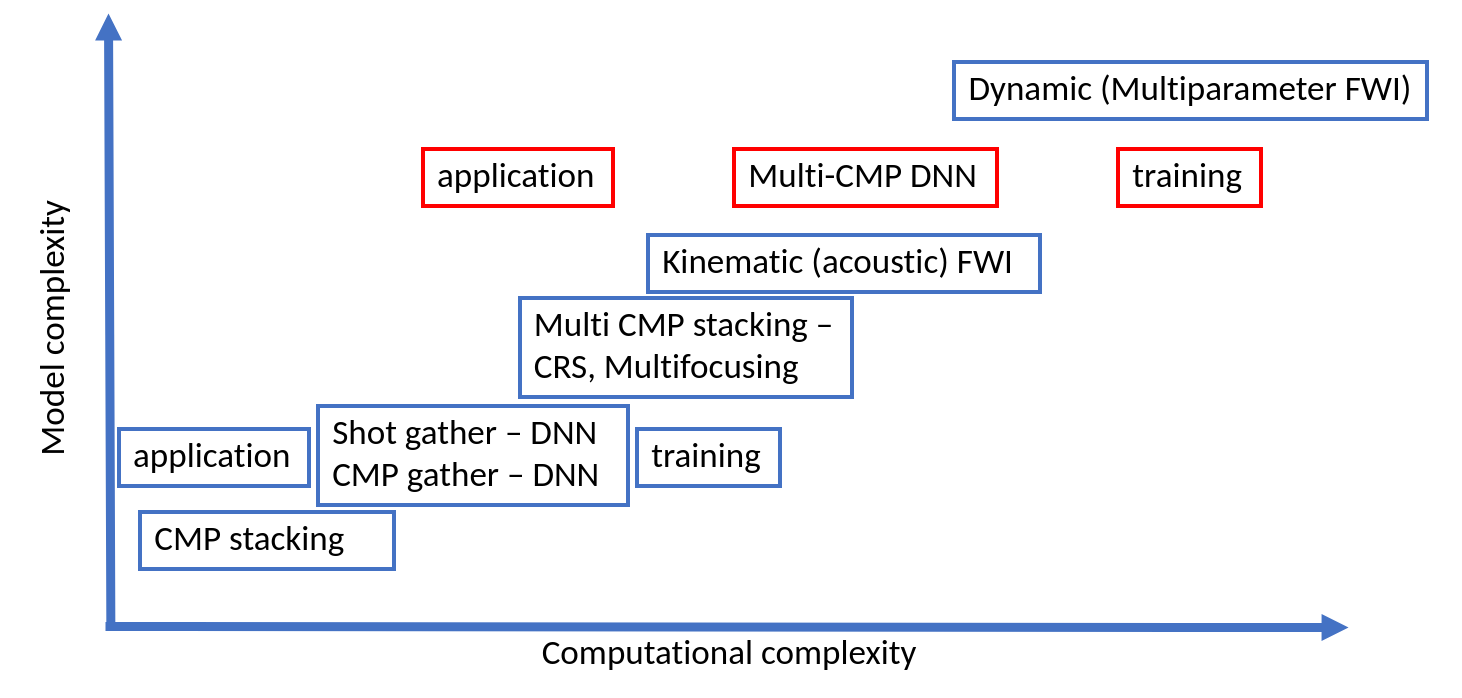
\includegraphics[width=0.9\linewidth]{Fig/learningParadigm}
	\caption{Deep learning is rather intensive in the training part, however the application of the trained deep neural network (DNN) is nearly instant}
	\label{fig:learningParadigm}
\end{figure}

% what shall we change?
Full waveform based methods listed above usually do not exploit the regularity of active seismic exploration sampling. Deep learning, on the other hand, can infer mapping for seismic data into the subsurface at a given location and then reapply it at another location. Most often attempts are made to infer models as a whole \citep{richardson2018seismic, wu2018inversionnet, zhang2018velocitygan, yang2019deep, oye2019velocity}. Here we propose to isolate, relevant to a given location data first and then try to map those into a single vertical velocity log. This set up effectively reduces the dimensionality of the target model space and simplifies the learning procedure. We also expect the learned NN to be more versatile for applications to other models since it corresponds to predicting a log, not a full model.
%Other available information in the form of well logs is also not normally utilized. 
%We will show how to build realistic models for deep learning training from these logs. 
% and  
%We believe that the computational efficiency of training can be improved by exploiting the regularity of conventional seismic sampling.

% how can we utilize the regularity of seismic sampling?
The paper is organized as follows. First, we discuss the regularity of sampling and seismic data relevance.
%
Then, we construct synthetic subsurface models for training purposes by using elastic and affine transforms of an existing model.
%
After that, we explore single-CMP versus multi-CMP training of a CNN and its application on the models that laterally vary very slowly.
%
Later we show that single CMP fails for geological models that vary laterally and we fix the problem with a multi-CMP setup.
%
Finally, we try to estimate the domain of applicability of the multi-CMP CNN and draw conclusions.



%Our solution belongs to the last class of methods too.
%
%
%
%One particular feature of exploration seismic data that is underutilized in FWI and and waveform based velocity model building tools is that the data are typically regularly sampled. Tis means that the inversion in different locations may be revealing very different subsurface structures but the data are aquired in the same way. The most straightforward way to acknowledge the data feature is through 1D assumption. \cite{roth1994} mapped shot gathers into 1D velocity profiles and \cite{zheng2019} mapped CMP gathers into velocity logs. It would be unfair to expect more complicated structures to be revealed from single CMP gathers. Here we show the limitations of single CMP mapping and propose an extension to multiple CMP gathers, that allows us to accomodate later variations in the model.
%
%
%
%
%
%
%
%
%
%
%Without prior assumptions inversion is very ill-posed and non-unique.
%
%% how is it typically handled?
%
%
%
%
%Typical way of tackling the non-uniqueness is by introducing a regularization term into inversion. With deep learning it is also possible, but there is another opportunity to just design models that are realistic (satisfy the prior assumptions) for training of the network. 
%
% 
%Deep learning is not new to seismic inversion \citep{roth1994}, yet it emerged main stream in the very past years. Several recent applications claim to yield good results, yet most of the models revealed with the help of deep learning are relatively simple and unrealistic. Here we show that neural networks can be applied to obtain models with fine features and realistic structures.
%
%this brings efforts low frequency extrapolation, low wavenumber estimation, initial model building and FWI modifications (citations). With all these pogosticks FWI usually works, yet gives to major computational costs, which makes it less appealing than conventional velocity analysis or it's more advanced spin-offs (CRS, multifocusing). Here we propose a deep learning based model for the inversion of seismic waveforms that combines the promise of FWI with the efficiency of conventional velocity analysis.
%
%\textbf{
%The paper is organized according to the following structure:
%we first estimate physical limitations to the resolving capabilities in the data, coming from wavenumber illumination theory.
%Then we introduce the data set with a focus on building a set of realistic velocity models for the training set. 
%After that we introduce and discuss the neural network architecture.
%Finally we perform training and apply the neural network to several data sets.
%}
\section{Regularity and relevance of seismic data}
Equidistant placement of active seismic sources and receivers in active seismic acquisition helps to balance illumination of the subsurface, easier to design and process with conventional stacking procedures. Regular sampling is therefore typical in active seismic exploration. Thus, for the common midpoints (CMPs), in the middle of the region of interest, the set of available offsets typically is the same.
This means that the setup for predicting the velocity profile can be the same for different CMPs.
The last fact is acknowledged by conventional velocity analysis such as Dix conversion, and advanced stacking procedures \citep{mann1999common}. However, to the best of our knowledge, these procedures rely on significantly simplified assumptions about the subsurface and do not perform well in complicated geological scenarios.
FWI, on the other hand, can accommodate arbitrary model complexity, yet forgets about the regularity of the sampling and spatial relations between model data are typically handled implicitly. Data-driven inversion will allow us to construct a CNN that maps relevant data to relevant location, and disregards the irrelevant data.  

\subsection{Relevant data}

First, let us examine the potential contribution expected from seismic data to a particular subsurface location illumination.

\begin{figure}[h!]
	\centering
	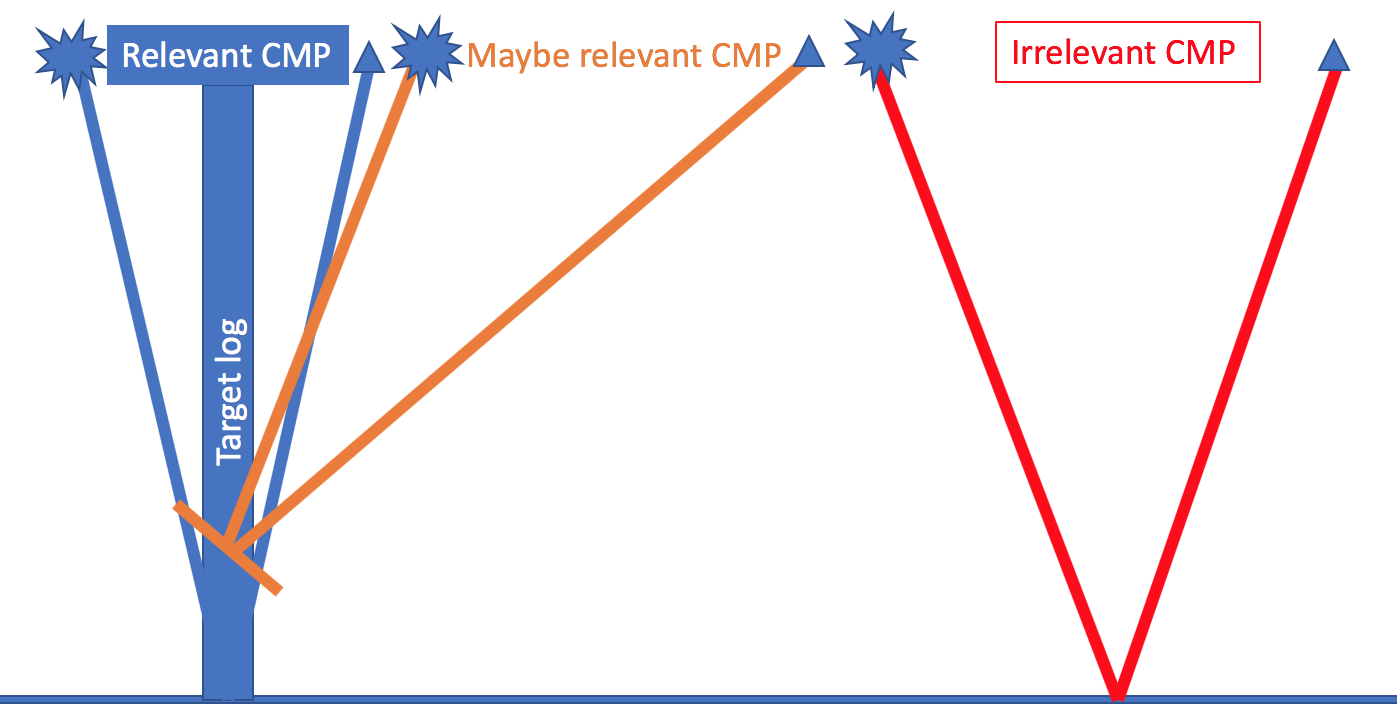
\includegraphics[width=0.7\linewidth]{Fig/relevantCMP}
	\caption{Relevant common midpoint (CMP) gathers - right above the image point location are utilized by standard stacking procedures and FWI. The gathers that are slightly shifted may also be useful in laterally heterogeneous media, but they are often discarded. CMP gathers that are far away from the imaging point are not spatially related to the imaging point, we discard those from the input}
	\label{fig:relevantCMP}
\end{figure}

Standard velocity analysis uses CMP stacking along hyperbolas to extract velocities and then the stacked data are mapped to depth. This obviously is good enough for horizontally layered media in most cases. More advanced velocity analysis techniques such as common reflection surface  \citep{mann1999common} or multi-focusing \citep{gelchinsky1999multifocusing}, take care of mild horizontal velocity variations and curved reflectors relying on certain assumptions about the subsurface. We take this concept to its extreme by relying on geologically plausible models as realistic scenarios and replacing the conventional stacking analysis with deep learning inference.

In particular, we construct CNN that is trained to perform mapping of relevant seismic data cubes to respective velocity logs, shown in \figref{in_out}: 
\beq \label{eq:mapping}
u_{obs}(x_{CMP}-\varepsilon:x_{CMP}+\varepsilon, h_{min}:h_{max}, :) \to v(x_{CMP}, :).
\eeq
Relevant observed data $u_{obs}(x_{CMP}-\varepsilon:x_{CMP}+\varepsilon, h_{min}:h_{max}, t)$  
to an estimate of velocity at target location $v(x_{CMP}, z)$, $x_{CMP}$ is the central midpoint,
$u_{obs}$ is the observed wavefield (acoustic pressure in our case). Here $x_{CMP}$ is the target vertical seismic velocity profile, $h_{min}$ and $h_{max}$ are the shortest and the longest offsets that are usable from the data, $t$ and $z$ stand for time and depth, respectively.

In the next subsection, we discuss why the mapping defined by \eqrf{mapping} is a candidate for an optimal way to cast seismic exploration inverse problem in the deep learning set up.  
\begin{figure}[h!]
	\centering
	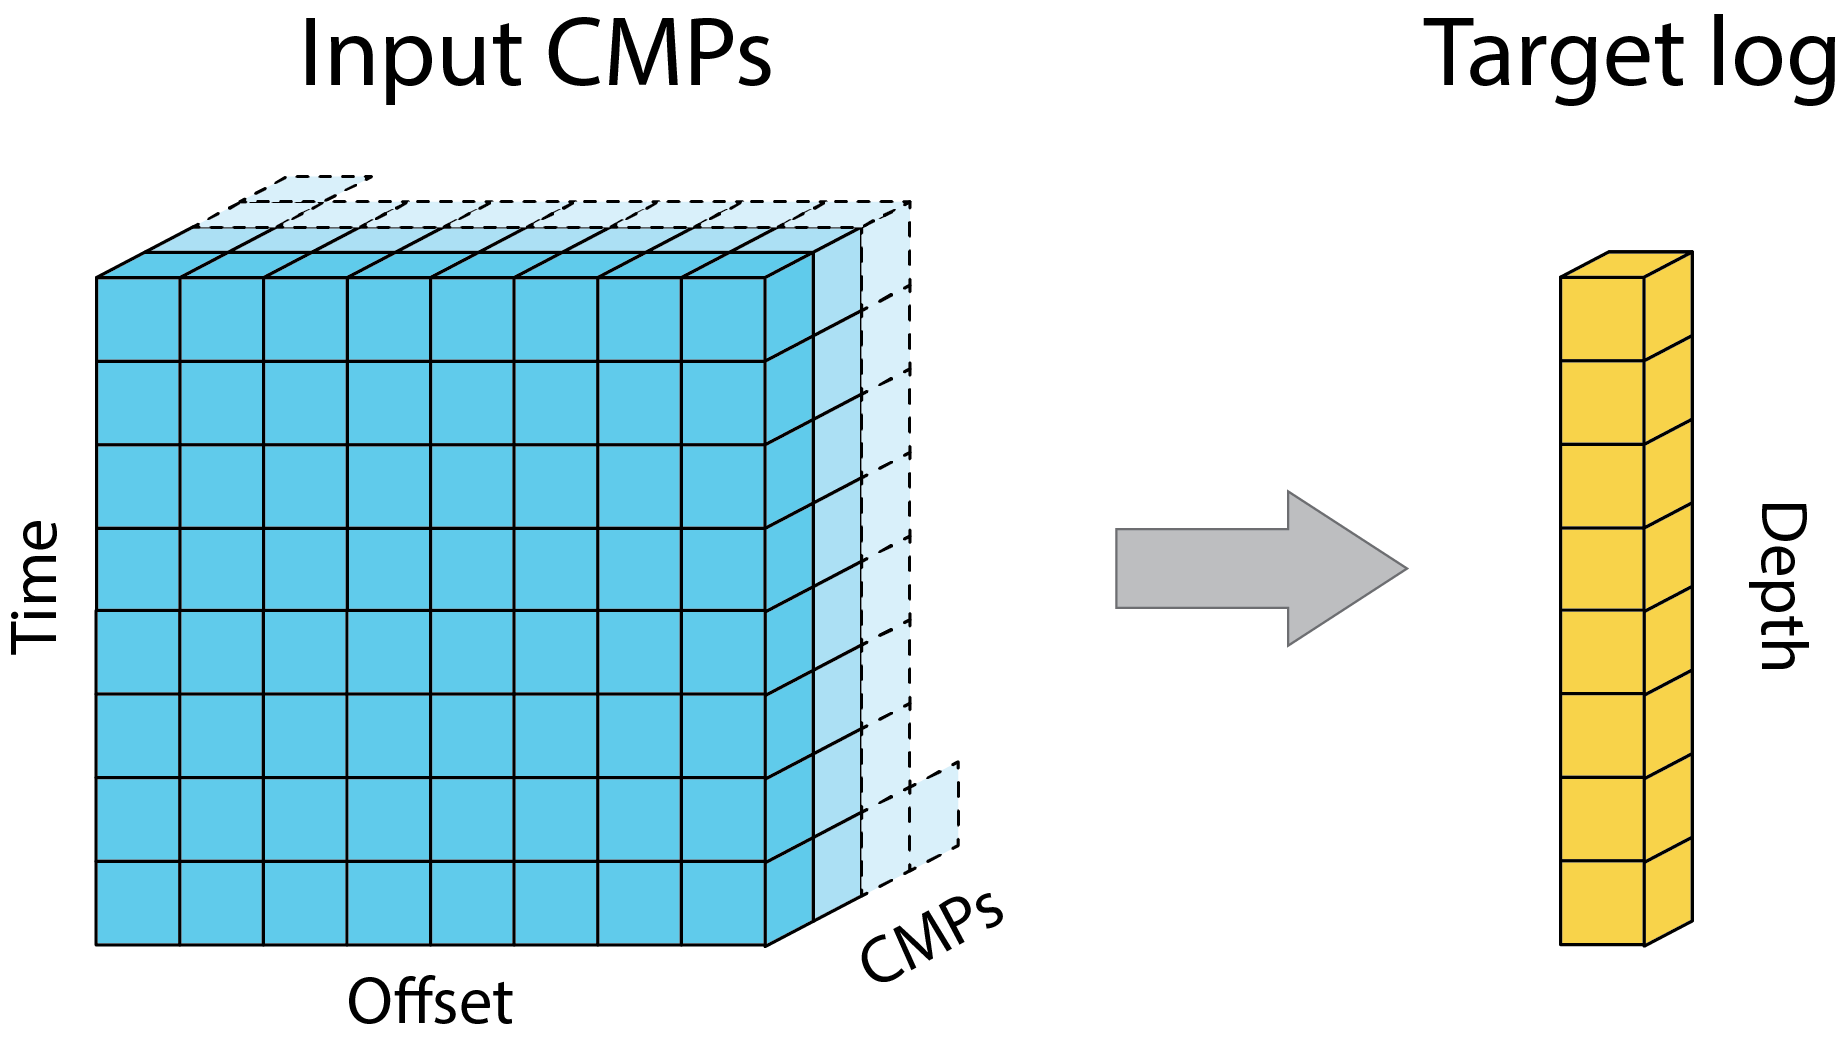
\includegraphics[width=0.7\linewidth]{Fig/in_out_shape}
	\caption{A set of neigboring CMP gathers is mapped to a velocity vertical profile with its horizontal coordinate corresponding to the middle of this set.}
	\label{fig:in_out}
\end{figure}

\subsection{Regularity of seismic data and deep learning inversion of full-waveforms}

Conventional active seismic acquisition aims at providing equal illumination to all the target areas of interest. Since the Earth's subsurface parameters are not known, we often accomplished this objective by setting up a survey that is regularly sampled in all available dimensions. Therefore the problem of vertical velocity profile estimation is exactly the same regardless of the location for a given exploration field. Taking this fact into consideration, we can set up an ML problem that takes advantage of similar data coverage for all locations. 

The resemblance between different locations in the field of exploration is rather well understood and taken into account in seismic imaging methods that rely on simplified media assumptions, such as stacking. It, however, can not be easily incorporated into full-waveform modeling based methods such as FWI and reverse-time migration (RTM).   
%
Artificial neural networks (ANNs) can serve as universal estimators, and have no principal constraints on which data space to map. Therefore, ANNs can be utilized to infer the mapping~\eqref{eq:mapping} from full-waveform modeling based methods. 

Finally, training deep neural networks is typically computationally expensive. From the mathematical point of view mapping~\eqref{eq:mapping} is a mapping of 3D functions (5D for 3D data acquisition) on compact to 1D functions, which should theoretically be much easier to estimate than mapping of full data to full models which would need inference between 3D and 2D functions in 2D problems, or even in 5D to 3D, for 3D problems. This makes the mapping to 1D logs an affordable and sufficient option.

%The regularity of conventional seismic exploration data and exploit the standard extended velocity analysis approach.

\section{Data}
Data-driven applications heavily depend on the quantity, features, and variability of samples in the dataset, which makes data collection and selection crucial. 
%
We intend to produce virtual well-logs from seismic data arranged into common-midpoint gathers. The dataset for such applications should consist of input seismic data and respective target logs. However, there are a very limited amount of field samples of well-logs because drilling and collection of cores is a costly task. 
%
To overcome this limitation we generate a synthetic dataset representing real-world geological features. First, we generate a set of random initiations of the subsurface models and then numerically propagate seismic waves in them. Later, recorded wavefields are assembled into CMPs and the random velocity models are decomposed into a set of well logs.

\subsection{Pseudo-random models}
Despite the clarity of intention, there is still no recognized way to generate realistic, textured all-purpose subsurface models with proper geological features.
%
Essentially, we combine elastic image transformations commonly used in text recognition applications \citep{simard2003best} and cropping with stretches \citep{sunLowFrequencyExtrapolation2018} from an existing model. More realistic subsurface models could potentially be delivered by using neural networks \citep{ovcharenko2019style} and wavelet packets \citep{kazei2019realistically}. However, to reduce ambiguity in model generation, multiple approaches and set ups need to be further tested.

%
In particular, we empirically generate pseudo-random subsurface models in three steps from the guiding model -- Marmousi benchmark model \citep{marmousi1991}.

\begin{itemize}
	\item First, we build the geological prior by flipping and replicating the Marmousi model (\figref{shiftsVectors}).
	
	\item Then, we produce a distortion map from a random Gaussian field (\figref{shiftsVectors}) and map vertical coordinates in the prior according to this field \figref{deformedModelNormal}.
	%We then stretch coordinates further \figref{deformedModelNormal}.
	
	\item Finally, we crop a random rectangular patch from the deformed model and resize it back to the size of the target subsurface model (\figref{random_model_example}).
\end{itemize} 



%\dplot{stretchMarm}{stretchMarm_strip}{To generate a pseudo-random model with realistic structures we first (a) flip and replicate Marmousi. (a) Full prior model. (b) Crop of the prior with dimensions similar to the original Marmousi II model.}

\dplot{shiftsVectors}{deformedModelNormal}{Generation of random subsurface models. Black arrows show vertical shifts (horizontal component added for better visualization) defined by random Gaussian field and applied to the geological prior -- guiding model. Guiding model before the transformation -- (a) and after the transformation -- (b). The coordinate transformation changes the order of some layers in the model, creates new layers and removes some of the other layers}
%Random Gaussian field defines (a) vertical shifts that we apply to the model. (b) deformed model

\aplot{random_model_example}{width=0.7\columnwidth}{An example of generated pseudo-random model.}


%\paragraph{Generator features}
The generator described above allows us to generate a set of models, which to some extent mimic the layered geological structure from the Marmousi model. Despite using a specific velocity reference, the generator produces a diverse range of subsurface models, which automatically satisfy the desired range of velocities. The main part of the transformation is local texture vertical repositioning. However, depending on the smoothness of the coordinate transformation, new horizontal layers can be generated and old layers may collapse.

\subsection{Seismic wave propagation}
There are no principal limitations to the type of wave equation or solver we may use. Yet, a few thousands of shots are necessary to generate statistically significant input for the machine learning. To reduce the computational cost of modeling acoustic 2D \citep{polo2018,ovcharenko2018,ovcharenko2019deep, li2019} or elastic 1D \citep[e.g.][]{zheng2019} media assumptions are typically utilized.

Should the model be horizontally invariant, we can try to reconstruct its elastic layers from a single shot gather \citep{roth1994}, or a single CMP gather \citep{zheng2019}.
While there is limited applicability of DL models to laterally inhomogeneous models \citep{zheng2019}, to the best of our knowledge, training was performed on vertically variant models to speed up the data generation. Here we utilize conventional finite-difference 2D wave propagation and investigate different options for laterally variant media.
Data are generated with equidistant sources and receivers at a spacing of 100m. The maximum offset is limited to 4km and the source central frequency is set to 7Hz, to present a decent challenge to conventional FWI.

To generate seismic data in each random model we integrate the Madagascar package \citep{fomel2013madagascar} into the workflow. 
We use a CUDA-accelerated acoustic finite-difference solver in the time domain to numerically simulate seismic wave propagation and to record seismograms at each receiver for every source in the acquisition.
%




% function "sfgenshots" - a cuda-based finite-difference solver. There are no principal limitations to the type of solver to be used. After that the shots are sorted into CMP gathers.

\section{Deep learning: Setup}
The general idea of deep learning is to build a mathematical model, which would derive a desired non-linear relation directly from the data. Selection of a particular DL model is heavily motivated by the attributes of the available data. 

%\subsection{Input and output}
%	supervised learning
We map multiple input CMP gathers (\figref{X_muted}) to respective target well-logs. Provided that the inputs and outputs are known, the problem reduces to multivariate regression. Therefore, the problem falls into the supervised learning setup.  

At the training stage, a supervised model attempts to derive a relation, which would link input and target variables for each pair in the training partition of the dataset. Whereas at the inference stage, the model infers target variables when given a sample from the previously unseen test partition of the data.

\subsection{Preprocessing}
Regardless of the type of DL models used in the application, a proper normalization is required for each sample of the input and target data. Normalization makes data fit the range matching the bounds of activation functions as well as it enforces even contributions of features into training. This leads to weight optimization (training) to a better convergence in a shorter time.

%Target data are seismic velocity profiles, those already have a range and have similar variability therefore standard Min-Max scaling to the into range $[-1, 1]$ works rather well for these data and does not change the patterns that can be extracted from those.  

The target data are seismic velocity profiles, which naturally span a narrow range of values and have similar variability. Therefore, common Min-Max scaling to the range $[-1, 1]$ enhances the target data representation while not changing the patterns that can be extracted from the logs.  

Input seismic data, on the other hand, require more complex geometric spreading correction to enhance the amplitudes of seismic event that carry the most useful information.
%
We empirically found that the Min-Max scaler from the Scikit-learn library \citep{scikit-learn}, applied to the set of samples, destroys spatial and temporal continuity in the data and leads to the subsequent poor performance of the neural network. On the other hand, data standardization with StandardScaler (linear scaling to unit variance and zero mean) preserves continuity in the data. After the standardization, we downscale the data with an empirically chosen coefficient of 0.1 and then mute the outliers to fit all the data into the [-1, 1] range (\figref{X_scaled}).

\dplot{X_muted}{X_scaled}{Input seismic data to the network. A raw CMP gather (a) and a scaled version of the same CMP gather (b). We utilize only positive offset as the data are synthetic and due to the reciprocity there is no difference with swapping source and receiver positions.}


\subsection{Convolutional neural networks (CNN)}
%   spatial dependency = convolutional
Regular feed-forward neural networks, such as multilayer perceptron, are suitable for problems with a relatively small size of input data as the number of parameters in them grows exponentially. When the input volume is an image then networks with convolutional layers come into play. Convolutional layers perform convolution of the input volume with a set of filters, which results in a set of feature maps, one corresponding to each filter respectively. The key feature of the convolutional layer is that it admits local connectivity. Meaning that when the filter slides over the input volume, only a small set of neighboring points contribute to a particular point of the feature map. This feature allows such a network to learn spatial patterns and enforce them at the inference stage.

Here, we consider two CNNs with exactly the same architecture, apart from the first layer, which will accept input data of the different shape.
%
First, we construct a 2D convolutional neural network that shifts its filters along offset and time for individual CMPs. This neural network takes a single CMP gather as input.
The second neural network takes multiple CMPs as multiple channels in the first layer and then follows exactly the same architecture as the first neural network (shown in \figref{architecture}).
The rectified linear unit activation function 
\beq
f(x) = max(x, 0)
\eeq
is applied to the output of every layer x but the last one. The last layer features a linear activation function, to fit the output scaled to the range [-1, 1]. This configuration is commonly utilized in DL applications as it presents a computationally cheap way to introduce non-linearity into the network. 
Finally, we apply 0.1 dropout to every layer in order to regularize the training process and prevent overfitting. 
%\subsection{CNN design}

\aplot{architecture}{width=\linewidth}{Purely convolutional neural architecture allows us to easily scale the input and output data. Maximum pooling layer and layers with strides larger than one provide compression of the data within the neural network. The last layer features large convolutional filter and essentially replaces a fully connected layer.}

%	Preprocessing
%		explain preprocessing
%	explaing perks of conv 
%	keras tensorflow




%Here, following \citep{york2019}, we generate the data and try to learn the respective logs.

\section{DL: Training}
Fitting within the CNN happens through the filters. First, CNN filters are initialized with random values and then those are optimized to match the output. The optimization is typically executed with a local search method through backpropagation of errors of the neural network on training data set. 
%The network is trained given the training part of the dataset whereas its performance is estimated by evaluation of inference result on the validation data. Final performance is measured from inference on testing data.

\subsection{Data splitting}
The learning process starts with splitting all available data into training, validation and testing subsets. 
The goal of training is
%not learning the input-output relation as a data base or dictionary, but 
to infer the dependence between input and target data in a way that it can further be applied to other data. Therefore, the performance of the CNN is evaluated throughout the process of training by applying the neural network to so called validation data. Once CNN stops improving its performance on the validation data set, the training stops. The validation data is utilized for monitoring the training process and should not be used for evaluating the model performance.   Thus, a small portion of the whole data is isolated from the training procedure to form the test data set. 

Often the three subsets of the data are determined randomly, yet it is not fair in our case since samples are spatially correlated. If CNN has seen neighboring logs in the training all it learns would be simple interpolation between them. To mitigate this problem in the testing of the neural network performance and in order to be able to examine performance on training samples we split the data set in the following way. We extract the last 10\% of samples and split them into 5\% for testing and 5\% that are always used in training that we perform throughout the paper. These 10\% of the data we later on utilize to visually inspect the fitting for training and testing samples. The rest, 90\% of the data are split according to Pareto principle \citep{dunford2014pareto} into training and validation sets randomly (\figref{T_data_split}).


\subsection{Optimization}
Once the training set is organized we need to choose the optimization strategy. This typically includes an optimization algorithm and its parameters. We use Nadam \citep{dozat2016incorporating} -- adaptive moment estimation (Adam) enhanced by Nesterov accelerated momentum. We empirically find that a batch size of 32 provides high, yet still stable performance over epochs in our case for about 30.000 samples. Nadam provides rapid decrease in the loss function and we notice that the validation loss essentially stops decaying in about 20 epochs for both neural networks  (\figref{singleCMP_loss_Full}). Then the learning rate is decreased to further fit the data. Both DNNs tend to overfit the data, which to some extent is prevented by early stopping. Training takes about 5 seconds per epoch for the single CMP neural network and about 45 seconds for a single epoch for multi CMP neural network. The training time is governed by the large filter sizes in the first layer of the neural networks and larger number of input channels in the case of the multi CMP DNN. Wiener filters commonly used for preprocessing of seismic data before inversion \citep{claerbout1985fundamentals} inspire us to have larger filters in the first layer of the network. 

\dplot{singleCMP_loss}{multiCMP_loss}{Loss functions on training and validation partitions of the dataset. Single CMP training (a) and multi-CMP training (b).}

\subsection{Evaluation}
After training we can visually evaluate the performance of CNNs on the training and testing subsets of the initially generated data. Comparison of training results of single CMP CNN (\figref{train_singleCMP_predicted}), multi-CMP CNN (\figref{train_multiCMP_predicted}) and ground truth (\figref{train_multiCMP_true}) shows that both neural networks fit training data set fairly well, with mildly better fit by the multi-CMP CNN. Also both neural networks seem to work well for the near-surface area in the models up to about 500m depth on testing data set. On the other hand the deeper structures are not that well revealed. Note, however, that taking into account the limited offset and central frequency of the wavelet conventional FWI would also probably fail for the deeper parts. %\todo{Quantitative comparison? Add any numbers}

\fplot{T_data_split}{train_singleCMP_predicted}
{train_multiCMP_predicted}{train_multiCMP_true}{(a) Training set is split into: training, testing and validation parts. (d) Last 10\% of the data set. First 5\% are used in training and the last 5\% are not. (c) and (d) Predicted velocity logs by single CMP data and from multi CMP data.}

\subsection{Reproducibility}
One of the main features of the neural networks is their stochasticity. There are multiple reasonable mappings that the neural network could learn in a multidimensional regression setting. Leaving the randomness of our training data set out of scope (we fix the seed for reproducibility of the data set) stochasticity of the neural networks comes from several factors: random weight initiation, random training set shuffling, random parallel arithmetic operations order inside the GPU. While the first two factors could in principle be isolated by random seed selection, the third one is very hard to deal with. Apart from that, particular choices of random initial weights should not significantly affect the inversion results.

Therefore, instead of going for exact numerical reproducibility we try to provide a clue about the randomness of our estimates by training multiple instances of our neural networks on the same data set. In order to keep the computational time within a few hours we take only five instances of each network, which is not enough to get a reasonable uncertainty estimate but it can provide us with some insights into it. In the next section, we test our trained ensembles of five CNNs each.

\section{DL: Applications}
In most deep learning applications to seismic inverse problems, the models are significantly simplified. Here we go for the full model complexity. The section consists of several synthetic tests and is organized with increasing true model complexity. We start with a pseudo-1D model generated by a horizontal stretching of the guiding model, then by random deformation of that model, which is still for the most part horizontally layered. After that, we apply our inversion to the guiding Marmousi model itself. Then we examine the application to a rescaled crop from the SEAM model. Finally we show applications to Overthrust model and its pseudo-1D derivative. In every case, we apply five trained instances of each (multi-CMP and single-CMP) CNN type. Finally, for each CNN type, we compute the average and standard deviation of the outputs within the respective ensemble.

%% figure naming convention:
%(train/test)_(prefix(singleCMP/multiCMP))_{folder(for train: ""=x1,x2,x3:marmvel1D, marmvel1D_distort,marmvel,overthrust1D,overthrust2D)}_{inverted/true/X_scaled}

\subsection{Guiding model and its derivatives}

Despite the diversity of pseudo-random subsurface models used for training, these are still biased toward the guiding model which has been selected as prior. The purpose of this section is to investigate the behavior of the deep learning model when applied to different scenarios derived from the original guiding model.

\paragraph{Marmousi 1D}
\newcommand{\modelFname}{marmvel1D}

The first question that we would like to answer is if the CNN that we trained can fit part of the stretched Marmousi model (\figref{test_singleCMP_\modelFname_true}), yet was not used in training directly. \figref{test_singleCMP_\modelFname_true_Full} shows the results of inversion for synthetic data acquired in such a model. Data in this case are not significantly clipped (\figref{test_multiCMP_\modelFname_X_scaled}) and do not vary significantly between multi-CMP input channels. The input of multi-CMP CNN is largely redundant as the model is essentially 1D. Therefore as expected CNN utilizing single CMP input is performing better (\figref{test_singleCMP_\modelFname_inverted}) than the multi-CMP CNN (\figref{test_multiCMP_\modelFname_inverted}). This fact is also reflected in the standard deviation maps (\figref{test_singleCMP_\modelFname_inverted_std_dev} and \figref{test_multiCMP_\modelFname_inverted_std_dev}). Standard deviation maps describe inconsistency between log predictions by five identical but independent networks. These were trained by starting from different weight initializations and thus converged to slightly distinct final results. The ensemble of CNNs is obviously not sufficient to estimate variance properly, yet we notice that the variance is increasing with depth and is focused around the deeper high-velocity layer location.


\splot{test_singleCMP_\modelFname_true}{test_multiCMP_\modelFname_X_scaled}
{test_singleCMP_\modelFname_inverted}{test_multiCMP_\modelFname_inverted}
{test_singleCMP_\modelFname_inverted_std_dev} {test_multiCMP_\modelFname_inverted_std_dev}
{(a)Test model -- stretched crop from the left edge of the Marmousi model. (b) Rescaled CMP gathers used as the first and the last channels of an input sample of multi-CMP CNN. Average prediction from the ensemble of (b) -- single-CMP CNNs and (c) -- multi-CMP CNN. Standard deviation for the (d) -- single CMP CNN outputs, (e) -- multi-CMP CNN outputs. }

\paragraph{Distorted Marmousi 1D}
\renewcommand{\modelFname}{marmvel1D_distort}
The second question is if the trained CNN would fit another model generated from Marmousi 1D by an elastic transform. While the guiding model is for the most part horizontally layered, large coordinate shifts create lateral variations (\figref{test_singleCMP_\modelFname_true}). We notice that shallow laterally varying anomalies can to some extent be estimated by both CNNs (\figref{test_singleCMP_\modelFname_inverted} and \figref{test_multiCMP_\modelFname_inverted}). Standard deviations within ensembles (\figref{test_singleCMP_\modelFname_inverted_std_dev} and \figref{test_multiCMP_\modelFname_inverted_std_dev}) suggest that the deeper part is not very well resolved by both CNNs. The shallow parts of the model are resolved rather well and the largest uncertainty is focused at the interfaces of shallow anomaly in the left part of the test model. Data representative in this case is not clipped much and shows visible amplitude variation between multi-CMP channels (\figref{test_multiCMP_\modelFname_X_scaled}).

\splot{test_singleCMP_\modelFname_true}{test_multiCMP_\modelFname_X_scaled}
{test_singleCMP_\modelFname_inverted}{test_multiCMP_\modelFname_inverted}
{test_singleCMP_\modelFname_inverted_std_dev} {test_multiCMP_\modelFname_inverted_std_dev}
{Same as \figref{test_singleCMP_marmvel1D_true_Full}, but for distorted 1D profile from Marmousi model. (e) The lateral heterogeneity becomes obvious in the CMP gathers}


\paragraph{Original Marmousi}
\renewcommand{\modelFname}{marmvel}
Guiding model -- Marmousi (\figref{test_singleCMP_\modelFname_true}) was not directly added to the training set, but was used for the training set generation. It is largerly laterally heterogeneous, yet single CMP CNN provides a reasonable estimate (\figref{test_singleCMP_\modelFname_inverted}), which would probably be good enough for a subsequent FWI application. On the other hand some layers introduced into the inversion result by single-CMP CNN are artificial. We attribute it to the limited information contained in single-CMP data. Multi-CMP CNN corrects for the artifacts (\figref{test_multiCMP_\modelFname_inverted}). The standard deviation maps (\figref{test_singleCMP_\modelFname_inverted_std_dev} and \figref{test_multiCMP_\modelFname_inverted_std_dev}) suggest that multi-CMP neural network provides a better estimate in this case. In the shallow part of the model the multi-CMP CNN standard deviation (\figref{test_singleCMP_\modelFname_inverted_std_dev}) has lower amplitude. In the deeper part of the model, it is more focused around the interfaces.  

\splot{test_singleCMP_\modelFname_true}{test_multiCMP_\modelFname_X_scaled}
{test_singleCMP_\modelFname_inverted}{test_multiCMP_\modelFname_inverted}
{test_singleCMP_\modelFname_inverted_std_dev} {test_multiCMP_\modelFname_inverted_std_dev}
{Same as \figref{test_singleCMP_marmvel1D_true_Full}, but for the Marmousi model itself}

\subsection{Generalization tests on other models}

The properly trained neural network should exhibit generalization capability. Meaning that it should infer meaningful result when applied to unseen data. However, when the new input data is sufficiently different from the training data, the prediction is expected to be inaccurate. In this paragraph, we demonstrate three applications of the network to the data significantly different from the one in training dataset. The first application is for salt-induced SEAM Phase I model, which produces data with strong reflections inconsistent with CMPs produced by a non-contrast training data. Other two examples are for 1D and 2D Overthrust models which resemble the layered structure of subsurface models used for training, however with different contrasts and layer inclination.


\paragraph{SEAM}
\renewcommand{\modelFname}{seam100}
SEAM Phase I model features strong reflections inconsistent with CMPs produced by non-contrast training data. This leads to poor standard scaler performance and a lot of data samples get clipped among the deeper reflections (\figref{test_multiCMP_\modelFname_X_scaled}). On the other hand velocities in the very near surface are low and diving waves don't get scaled properly. Some salt-like bodies are generated when we crop from deformed Marmousi model and stretch the crops. All these factors suggest that the training data set would need to be better tailored to local geology, therefore, the inversion recovers only the velocity trends next to the salt and the salt boundary. FWI tailored to salt body inversion \citep[e.g.][]{esserTotalvariationRegularizationStrategies2016,ovcharenko2018,kalita2019regularized} would still benefit from such an estimate used as a starting model.

\splot{test_singleCMP_\modelFname_true}{test_multiCMP_\modelFname_X_scaled}
{test_singleCMP_\modelFname_inverted}{test_multiCMP_\modelFname_inverted}
{test_singleCMP_\modelFname_inverted_std_dev} {test_multiCMP_\modelFname_inverted_std_dev}
{Same as \figref{test_singleCMP_marmvel1D_true_Full}, but for the rescaled crop from the SEAM model. (b) Scaling performs poorly as the training data set didn't include similar models}

The central part of the deviation map dominates over the neighboring regions. The CNNs were not given a sufficient amount of data/models featuring salt bodies. Therefore, they are not able to produce logs with large homogeneous high-velocity segments. 

\paragraph{Overthrust model}


In order to further explore the generalization power of the trained CNNs, we test them on data that are modeled in a slice of the Overthrust model. Which is challenging for FWI due to its low-velocity layers squeezed in between high-velocity reflectors and also challenging for conventional layer stripping due to uplifts and faults that distort otherwise low-relief structure. We split the phenomena into two. First, we replicate low-relief part of the Overthrust model to test the layer stripping capabilities of the trained CNNs and then we test on the full model extended by replication and flipping.

\subparagraph{Overthrust 1D}
\renewcommand{\modelFname}{overthrust1D}

Shallower layers in this model feature low contrasts and velocity increases and then decreases (\figref{test_singleCMP_\modelFname_true}). The data \figref{test_multiCMP_\modelFname_X_scaled} scaling shows very strong first arrivals and very low amplitude reflections, which focuses inversion on the near-surface anomalies.
Both CNNs seem to get the top of the model right (\figref{test_singleCMP_\modelFname_inverted},
\figref{test_multiCMP_\modelFname_inverted}) and fail at the bottom part. Single CMP CNN fails in a bit more moderate way as expected for this low-relief model. Deeper layers are mispositioned, which is reflected in overall increasing standard deviations within the ensembles (\figref{test_singleCMP_\modelFname_inverted_std_dev} and
\figref{test_multiCMP_\modelFname_inverted_std_dev}). 

\splot{test_singleCMP_\modelFname_true}{test_multiCMP_\modelFname_X_scaled}
{test_singleCMP_\modelFname_inverted}{test_multiCMP_\modelFname_inverted}
{test_singleCMP_\modelFname_inverted_std_dev} {test_multiCMP_\modelFname_inverted_std_dev}
{Same as \figref{test_singleCMP_marmvel1D_true_Full}, but for the pseudo-1D model generated from Overthrust model}

\subparagraph{Overthrust 2D}
\renewcommand{\modelFname}{overthrust2D}
Finally, we test both CNNs on a slice from the Overthrust model (\figref{test_singleCMP_\modelFname_true}). The scaled data \figref{test_multiCMP_\modelFname_X_scaled} shows very strong first arrivals and very strong late reflections. Those reflections are most likely multiples and therefore it is very hard to train CNNs to position those properly. Similarly to the case of 1D profile from the Overthrust model, both CNNs seem to get the top of the model right (\figref{test_singleCMP_\modelFname_inverted} and
\figref{test_multiCMP_\modelFname_inverted}) and fail at the bottom part. According to the standard deviation maps  (\figref{test_singleCMP_\modelFname_inverted_std_dev} and
\figref{test_multiCMP_\modelFname_inverted_std_dev}) up to the depth of 1.5km we can trust the inversions. However, only some features of the complicated layering are retrieved. We still expect that the inversion results would be useful as a starting point for FWI.

\splot{test_singleCMP_\modelFname_true}{test_multiCMP_\modelFname_X_scaled}
{test_singleCMP_\modelFname_inverted}{test_multiCMP_\modelFname_inverted}
{test_singleCMP_\modelFname_inverted_std_dev} {test_multiCMP_\modelFname_inverted_std_dev}
{Same as \figref{test_singleCMP_marmvel1D_true_Full}, but for the 2D slice of the Overthrust model}

%From the last test we clearly see a rather obvious fact -- single CMP gather cannot be mapped into velocity log successfully without the assumption of laterally slowly variant medium. We believe that this is a good motivation to study the mapping of multiple CMP gathers.



\section{Discussion}

For regularly sampled seismic data acquisition that is typical in seismic exploration, the problem of full-waveform based velocity model building can be reduced to the search for mapping from 3D data (relevant traces) to 1D data (single velocity logs). This formulation is not a viable option for conventional FWI implementations as a velocity model needs to be optimized as a whole. Deep neural networks, on the other hand, are universal estimators and can be trained to map arbitrary input to target data samples as long as there is such a mapping. Therefore, training for the inference of particular velocity logs from data sets is a viable option for deep learning based velocity model inference.

For a DL application, it is beneficial to split the whole data set into relevant and irrelevant data to speed up training. Therefore, we extracted the data (CMP gathers) from the neighboring area to the target vertical velocity profile location. We tried to infer this relation between these data and the respective velocity logs by using CNNs. In particular, we constructed two CNNs to infer this relation between the data and the vertical velocity profiles and analyzed their capabilities.

The first CNN used single-CMP data as input, and the second CNN used multiple neighboring CMP gathers as input. We trained both neural networks on data modeled in augmentations of the Marmousi model by elastic deformations and cropping. The single-CMP CNN outperformed the multi-CMP CNN on laterally invariant models and models with mild velocity variations. On the other hand, the multi-CMP CNN had a better learning capacity and performed better on models with strong lateral variations. Both CNNs failed to construct a salt body, which suggests that the augmentations of the Marmousi model lead to limited capacity for generalization. So far we suggest that the same CNNs can be applied for geologically similar exploration scenarios. The training data set must be extended further to accommodate models that are geologically very different from the guiding model. 

The application of trained CNNs presented here takes less than 1ms per sample (CMP gather). Therefore, with these CNNs, velocity models can be built much faster than they are currently built. The velocity models would also be built automatically from raw recorded waveforms. The resolution of the built models is comparable to traveltime tomographic models rather than FWI models. However, the models built in this way will be useful as starting models for FWI. Several instances of trained neural networks naturally provide an ensemble of starting models for the FWI uncertainty analysis.

This paper is a reproducible document. All related code can be found at \\ \href{https://github.com/vkazei/deeplogs}{https://github.com/vkazei/deeplogs}.

\section{Conclusion}

Deep learning allowed us to predict the mapping between raw seismic data (multi-CMP gathers) and vertical velocity profiles. This mapping is represented by trained purely convolutional neural networks (CNNs). Namely, we trained CNNs to map the relevant data cubes to 1D velocity profiles, rather than full velocity models. This is a key feature of our method that reduces the complexity of the training process and opens an opportunity for direct usage of the sonic logs for velocity-model building with deep learning.
 
Just like full-waveform inversion our method relies on full-waveform modeling and utilizes all available data. Therefore, there are no principal limitations to the complexity of models that can be inverted. Just like in FWI some prior assumptions about the velocity model are necessary to mitigate non-uniqueness in seismic inversion. These assumptions can easily be incorporated into the training set. Every application of conventional FWI requires numerous forward problem solutions in order to perform the model optimization. Every new application of trained neural networks is nearly instant. Therefore, once the network is trained on a data set with particular prior assumptions, similar data sets can be inverted much faster than with conventional FWI, and with higher resolution information.



%Therefore, if a neural network is trained on sufficiently representative of the geologic region set of models it can potentially replace other full-waveform based velocity model building methods. bringing us one step closer to real-time velocity model building with uncertainty quantification.




%The mapping in the form of a trained CNN allows us to build velocity models directly from surface seismic data.


 
%We constructed and trained two purely convolutional CNNs that map the relevant data to 1D vertical velocity profiles. Multi-CMP CNN has better capabilities to learn complex models, while single-CMP CNN works better for velocity models with mild velocity variations. 




%Training of neural networks is a computationally intensive process. 
%


\section{ACKNOWLEDGMENTS}

We thank members of the Seismic Modeling and Inversion group (SMI) and the Seismic Wave Analysis Group (SWAG) at KAUST for constructive discussions. We also thank Saudi Aramco for support.
The research reported in this publication was supported by funding from King Abdullah University of Science and Technology (KAUST), Thuwal, 23955-6900, Saudi Arabia.
%
\newpage



%\append{Appendix example}



\newpage

\bibliographystyle{apalike}  % style file is seg.bst
\bibliography{zotero}

\end{document}